% Authors: Axel Wachtler, Joerg Wunsch, Matthias Vorwerk
% http://www.uracoli.de

\documentclass{beamer}
\usepackage{beamerthemeshadow}
\usepackage[ngerman]{babel}
\usepackage[utf8x]{inputenc}
\usepackage{graphicx}

\definecolor{slidyblue}{HTML}{527bbd} % lightblue headings from slidy

\newcommand{\Head}[1]{{\textbf{\textcolor{slidyblue}{#1}}}}

% \usetheme{Boadilla}

% \setbeamercovered{transparent}
% \beamertemplatenavigationsymbolsempty
\setbeamertemplate{footline}[frame number]
\setbeamertemplate{headline}{}

\title{Drahtlose Sensordatenerfassung und -verarbeitung mit Linux}
\author{Axel Wachtler, Jörg Wunsch, Matthias Vorwerk}

\begin{document}

% \frame{\frametitle{Intro}
% \begin{figure}
% 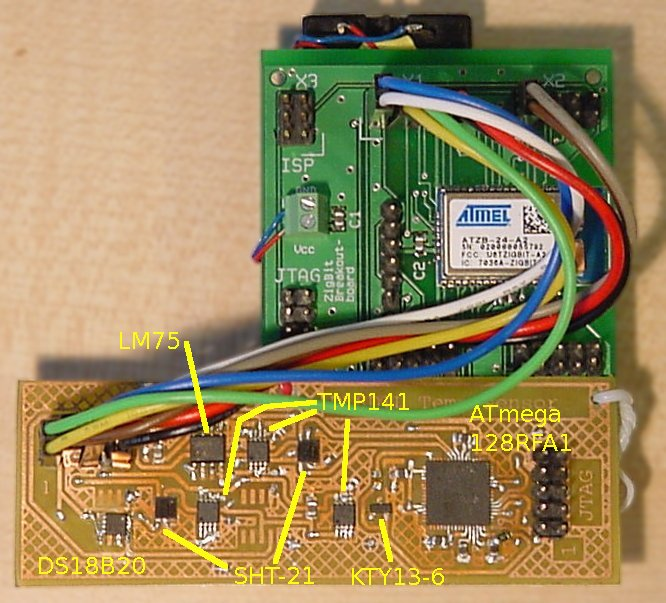
\includegraphics{../sensorboard.jpg}
% \caption{show an example picture}
% \end{figure}}

\frame{\titlepage}

% ----------------------------------------

\section{Einleitung}
\frame{\frametitle{Einleitung}
\Head{Motivation}
\begin{itemize}
\item<*> Umweltgrößen (Temperatur, Luftfeuchte, Druck und Licht) \textbf{beeinflussen technische Prozesse und Vorgänge als Stellgrößen}
\item<*> Durch die dezentrale Erfassung an (vielen) unterschiedlichen Orten kann der ortsabhängige Verlauf von Parametern bestimmt werden.
\item<*> Die \textbf{drahtgebundene} Verteilung von Sensoren verursacht einen erhöhten Infrastruktur-Aufwand.
\item<*> Die Datenrate einzelner Sensoren ist gering. Messwerte fallen in der Regel im Sekunden- oder Minutentakt an.
\end{itemize}
}

% ----------------------------------------

\frame{\frametitle{Gliederung}
\begin{itemize}
\item<*> Übersicht Funkmodule        		\pause
\item<*> Vergleich verschiedener Sensoren   \pause
\item<*> Verarbeitung der Sensordaten
\end{itemize}
}

% ----------------------------------------

\section{Drahtlose Sensornetzwerke}
\frame{\frametitle{Drahtlose Sensornetzwerke}%
\only<1>{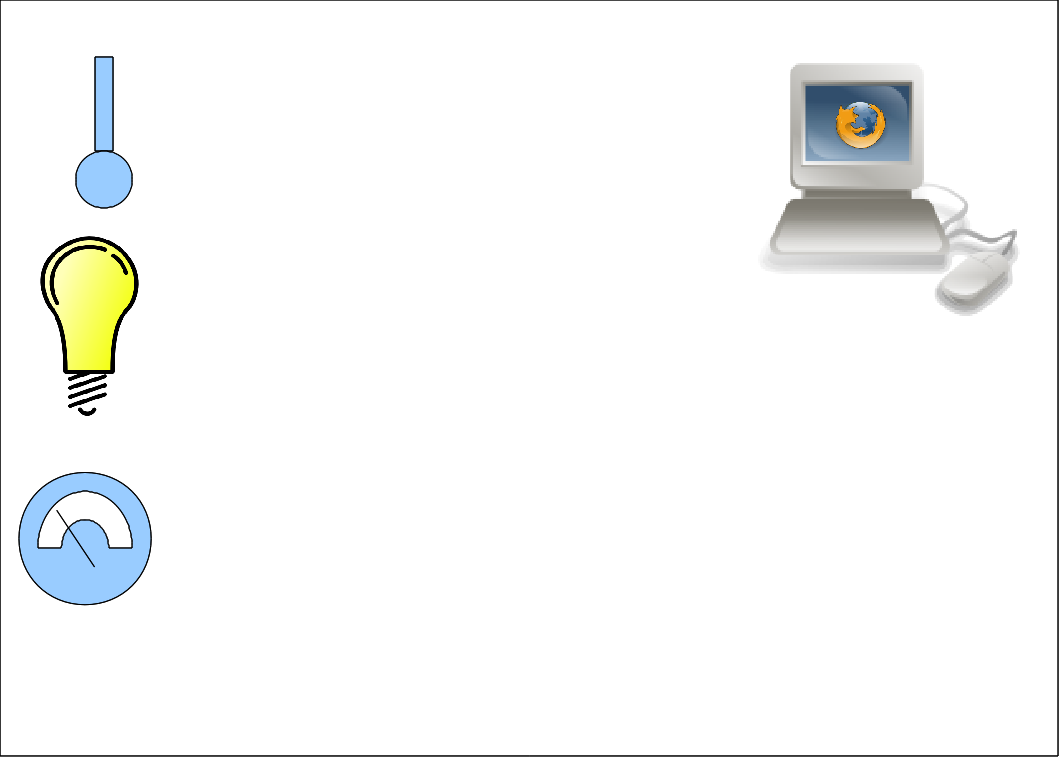
\includegraphics[width=0.9\textwidth]{../system_001.png}}%
\only<2>{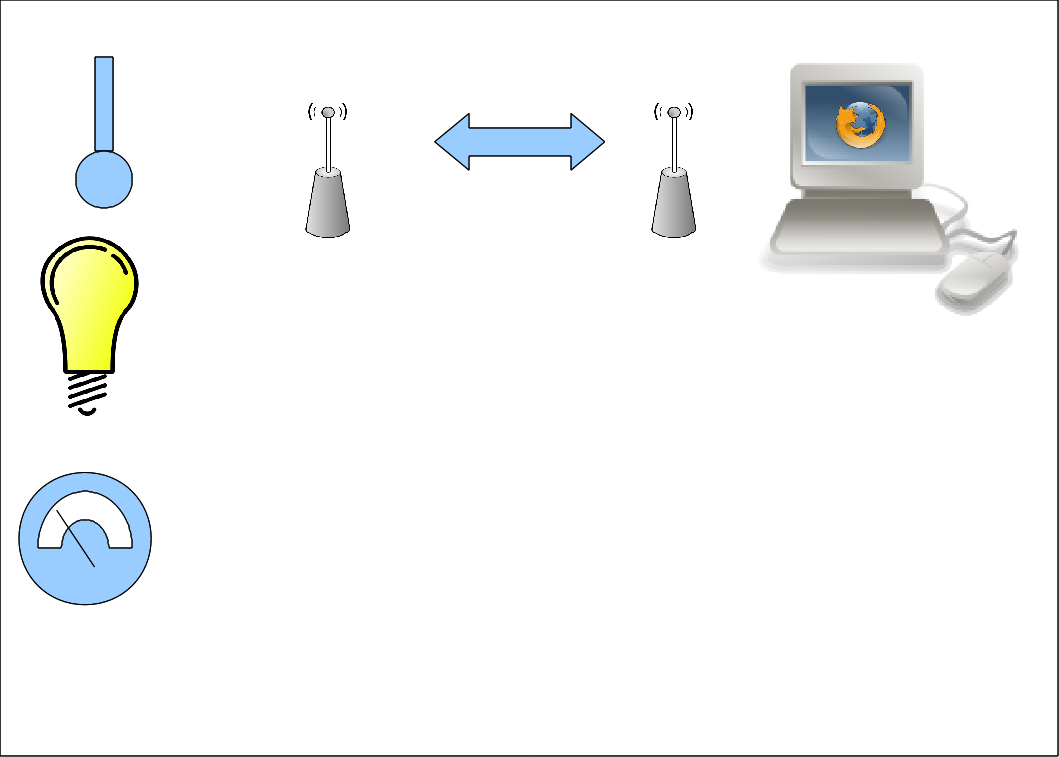
\includegraphics[width=0.9\textwidth]{../system_002.png}}%
\only<3>{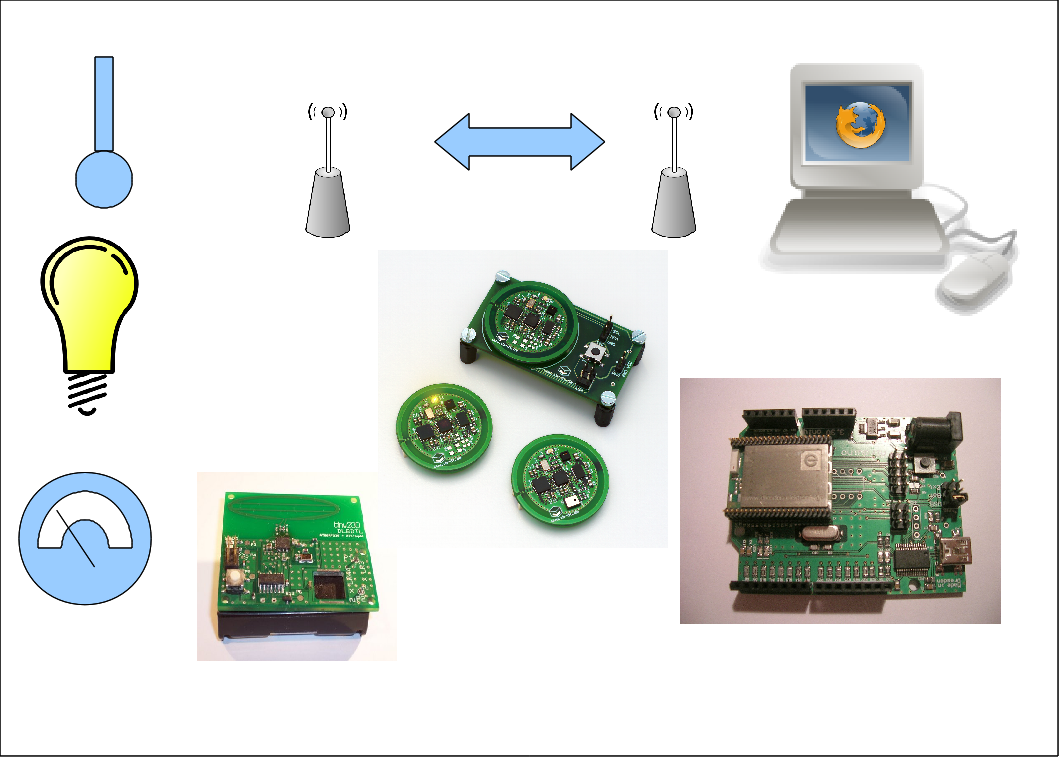
\includegraphics[width=0.9\textwidth]{../system_003.png}}%
}

% ----------------------------------------

\section{Funkstandards}
\frame{\frametitle{Funkstandards}
\begin{itemize}
\item<*> \Head{IEEE 802.11.x} (WiFi)         \pause
	\begin{itemize}
	\item 54 ... 300 Mbit/s
	\item Netzwerkinterface, FileTransfer, Audio, Video     \pause
	\end{itemize}
\item<*> \Head{IEEE 802.15.1} (Bluetooth)    \pause
	\begin{itemize}
	\item 732,2 kbit/s ... 2,1 MBit/s
	\item Nahbereichskommunikation, Sprachübertragung   	\pause
	\end{itemize}
\item<*> \Head{IEEE 802.15.4} (ZigBee)       \pause
	\begin{itemize}
	\item 20 bis 250 kbit/s
	\item hauptsächlich für Sensoranwendungen geeignet: 	\pause
 		\begin{itemize}
 			\item geringe Datenrate
 			\item energiesparend
 			\item niedrige Systemkosten
 		\end{itemize}
	\end{itemize}
\end{itemize}
}

% ----------------------------------------

\section{Drahtloses Datenlogger System}
\frame{\frametitle{Drahtloses Datenlogger System}
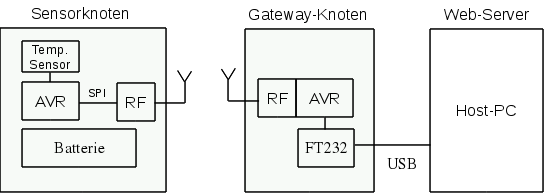
\includegraphics[width=\textwidth]{../blocks.png}
\begin{itemize}
\item \textcolor{slidyblue}{Sensorknoten}
	\begin{itemize}
	\item autark, (Batterie, Energy-Harvesting)
    \item sendet kontinuierlich die Werte der Sensoren zum Gateway
	\end{itemize}
\item \textcolor{slidyblue}{Gateway}
	\begin{itemize}
    \item Ausgabe der Sensordaten über serielles Interface
    \item permanente Stromversorgung (Netztteil, USB)
	\end{itemize}
\item \textcolor{slidyblue}{Webserver}
	\begin{itemize}
    \item liest und speichert die Daten vom Gatewayknoten
    \item Auswertung der Daten mit speziellen Anwendungen.
	\end{itemize}
\end{itemize}
}

% ----------------------------------------

\section{Boards}
\frame{\frametitle{Boards - Übersicht}

\begin{itemize}
\item Es gibt eine Vielzahl an Funkmodulen von unterschiedliche Boardherstellern.
\item Die µracoli-Library unterstützt derzeit über 30 Boards und Module
	\begin{itemize}
    \item A.N. Solutions
    \item Atmel
    \item Colorado Micro Devices
    \item Dietzsch und Thiele Partnerschaftsgesellschaft
    \item dresden elektronik ingenieurtechnik gmbh
    \item In-Circuit GmbH
    \item Logos Electromechanical LLC
    \item Meshnetics
	\end{itemize}
\end{itemize}
}

% ----------------------------------------

\frame{\frametitle{Boards - Vorstellung}
\begin{columns}
\column{.80\textwidth}

\begin{itemize}
 \item \textcolor{slidyblue}{tiny230} - DIY Projekt von \textbf{Jörg Wunsch}
	\begin{itemize}
    \item ATtiny44/84 mit AT86RF230/231,
    \item Sensoren: KTY13, LED als Lichtsensor
	\end{itemize}
 \item \textcolor{slidyblue}{RadioFaro*} - DIY Projekt von \textbf{Daniel Thiele}
	\begin{itemize}
    \item ATmega128RFA1 Module von Dresden Elektronik
    \item Arduino Formfaktor
	\end{itemize}
 \item \textcolor{slidyblue}{Muse231} - Prototyp, \textbf{Ingenieurbüro Dietzsch und Thiele}
	\begin{itemize}
    \item ATmega88PA + AT86RF231,
    \item Sensoren SHT21, MMA7455, Mikrofon, Lichtsensor-LED
	\end{itemize}
 \item \textcolor{slidyblue}{ZigBit Adapter Boards}
	\begin{itemize}
    \item ATmega1281 + AT86RF230
    \item Sensoren über Breakoutboard angeschlossen
	\end{itemize}
\end{itemize}
\column{.20\textwidth}
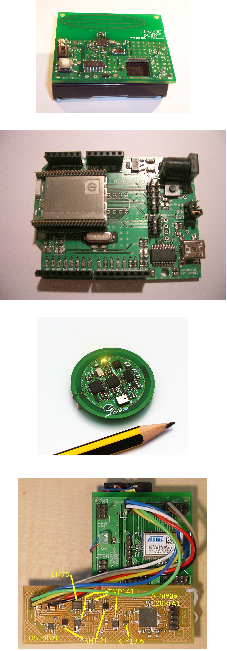
\includegraphics[width=\textwidth]{../hboards.png}
\end{columns}
}

% ----------------------------------------

\section{Zutaten für die Firmware-Entwicklung}
\frame{\frametitle{Zutaten für die Firmware-Entwicklung}
\Head{Hardware}
\begin{itemize}
 \item 1 x Gateway Knoten mit USB/RS232,  1...N x Sensorknoten
 \item 1 x Programmer, optional Hardware-Debugger
	\begin{itemize}
    \item AVR Dragon $\rightarrow$ ISP Programmer + JTAG Debugger
    \item AVR ISP, USBprog, PonyProg $\rightarrow$ ISP Programmer
    \item JTAG ICE mkII $\rightarrow$ JTAG Debugger
	\end{itemize}
\end{itemize}

\Head{Software}
\begin{itemize}
 \item  avr-gcc + binutils $\rightarrow$ Compiler und Linker
 \item  avr-libc $\rightarrow$ Standard C Library für AVR
 \item  avrdude $\rightarrow$ Programmier Tool
 \item  avarice + avr-gdb $\rightarrow$ Debugger und JTAG Bridge
 \item  µracoli $\rightarrow$ AVR Radio Library
\end{itemize}
}

% ----------------------------------------

\section{uracoli - Die AVR-Radio-Library}
\frame{\frametitle{µracoli - Die AVR-Radio-Library}
Library zur einfachen Inbetriebnahme von IEEE-802.15.4-Transceiver-Knoten.
\begin{figure}

\includegraphics[width=0.3\textwidth]{../uracoli-logo.png}
\end{figure}

\begin{itemize}
 \item  URL: http://www.uracoli.de           	\pause
 \item  derzeit über 40 Plattformen (AVR + Atmel-Transceiver) unterstützt    	\pause
 \item  High und Low Level Transceiver-Funktionen        	\pause
 \item  Timer, Sensor und IO-Funktionen sind optional      	\pause
 \item  viele Beispiele, Anwendungen: Wireless UART, Sniffer, Arduino Support  	\pause
 \item  modified BSD Lizenz
\end{itemize}

}

% ----------------------------------------

% sensor comparison slides

\section{Vergleich von Sensoren}
\frame{\frametitle{Vergleich von Sensoren}
\Head{Auswahl von Temperatursensoren} \pause

\begin{itemize}
\item große Vielfalt an analogen und digitalen Sensoren \pause
\item Vergleich von:
\begin{itemize}
\item LM75 (National Semiconductor, I²C)
\item DS18B20 (Maxim/Dallas, ``OneWire'')
\item SHT-21 (Sensirion (CH), I²C); Temperatur und rel. Luftfeuchte
\item TMP141 (TI/Burr Brown, ``SensorPath'')
\item KTY13-6 (Infineon)
\item ATmega128RFA1 (Atmel), interner Sensor \pause
\end{itemize}
\item Preis zwischen EUR 0,50 und EUR 20
\end{itemize}
}

% ----------------------------------------

\section{Versuchsaufbau}
\frame{\frametitle{Versuchsaufbau}
\begin{columns}

\column{.60\textwidth}
\Head{Hardware} \pause
\begin{itemize}
\item Montage der Sensoren auf Board
\item SHT-21 2x, TMP141 3x, alle anderen 1x
\item Abfrage über Zigbit-Funkmodul
\item Weiterleitung der Daten über Funk
\item Batteriebetrieb mit 2 x LR03
\end{itemize}

\column{.30\textwidth}
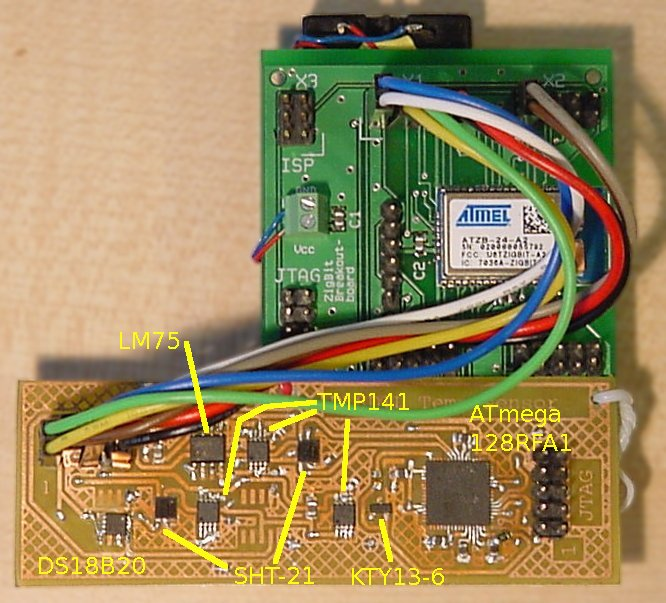
\includegraphics[width=\textwidth]{../sensorboard.jpg}\pause
\end{columns}

\vspace*{1.5em}
\Head{Umgebung} \pause

\begin{itemize}
\item Langzeittests in ruhiger Umgebung \pause
\item Vergleich mit Laborthermometer \pause
\item Tests in wechselnder Umgebung, einschließlich Klimaschrank Vötsch VT4004
\end{itemize}
}

% ----------------------------------------

\section{Messungen}
\frame{\frametitle{Messung in ruhiger Umgebung}
\only<2>{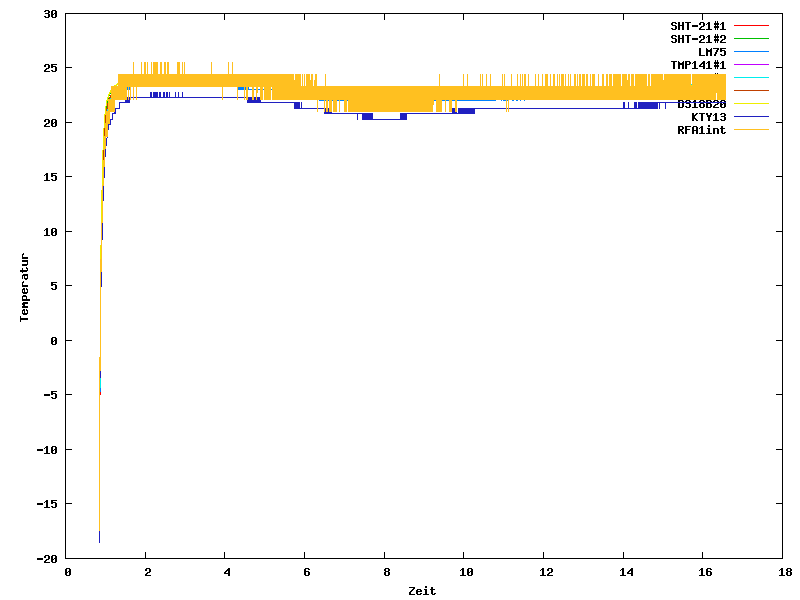
\includegraphics[width=\textwidth]{../all.png}}%}
\only<3>{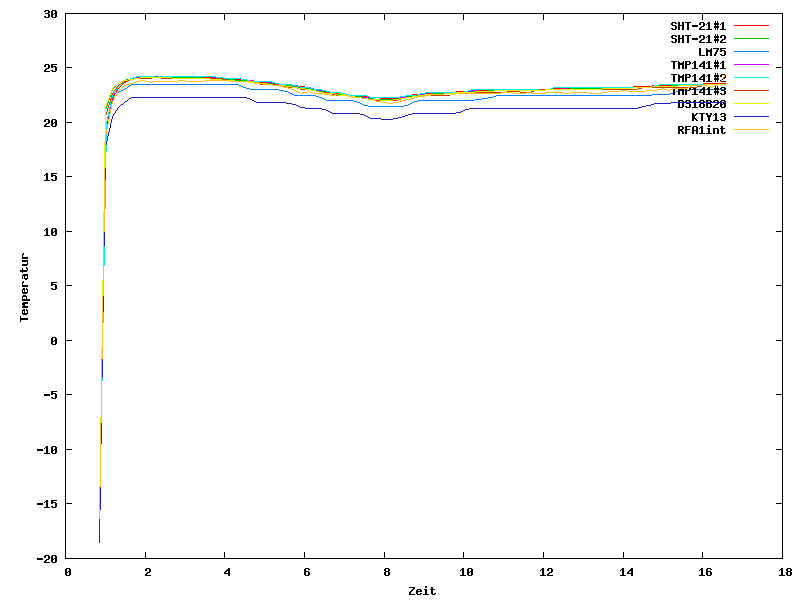
\includegraphics[width=\textwidth]{../smooth-all.png}}%}
\only<4>{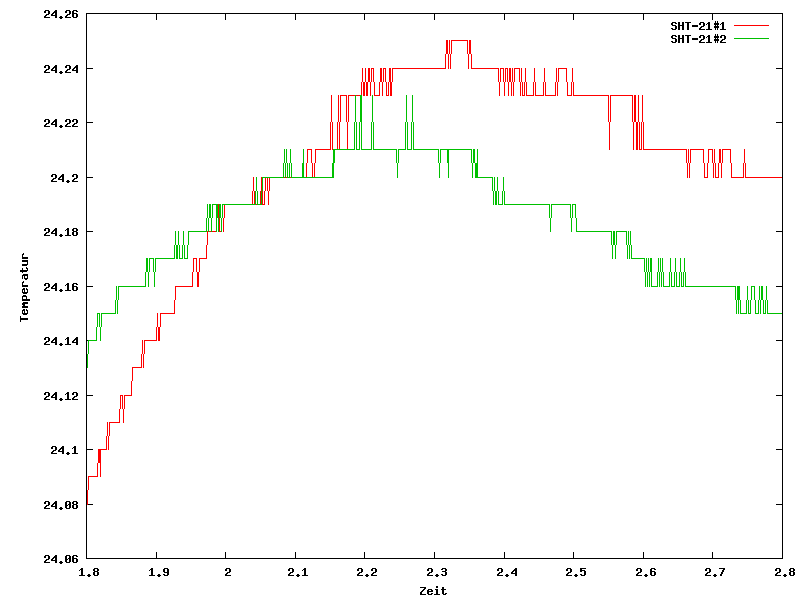
\includegraphics[width=\textwidth]{../nonsmooth.png}}%}
\only<5>{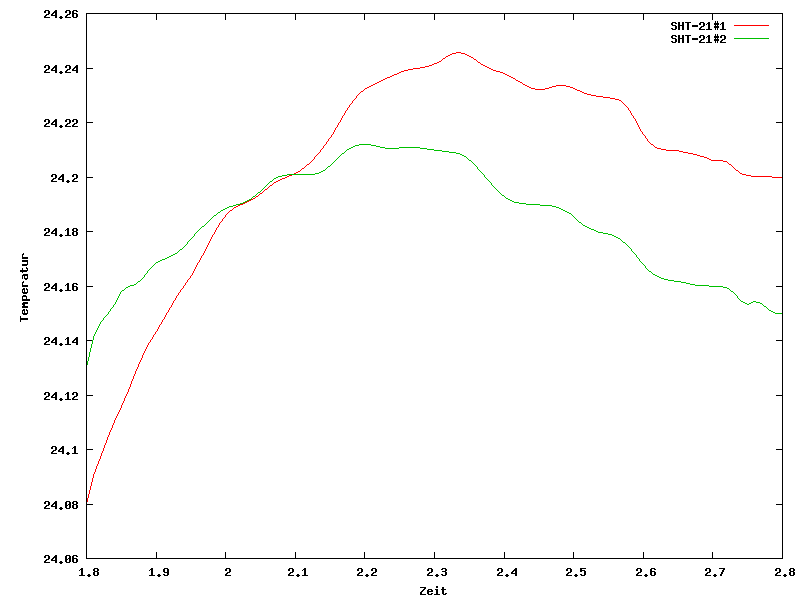
\includegraphics[width=\textwidth]{../smooth.png}}%}
\only<6>{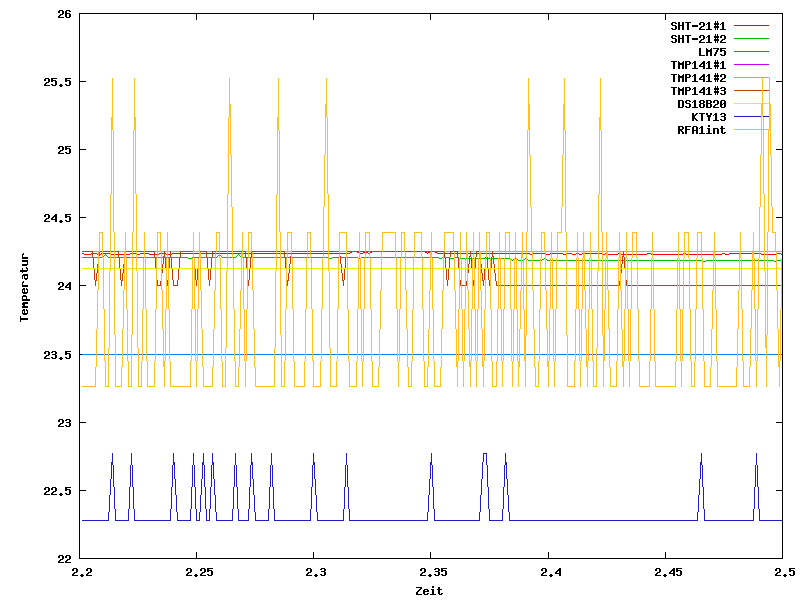
\includegraphics[width=\textwidth]{../stable.png}}%}
\only<7>{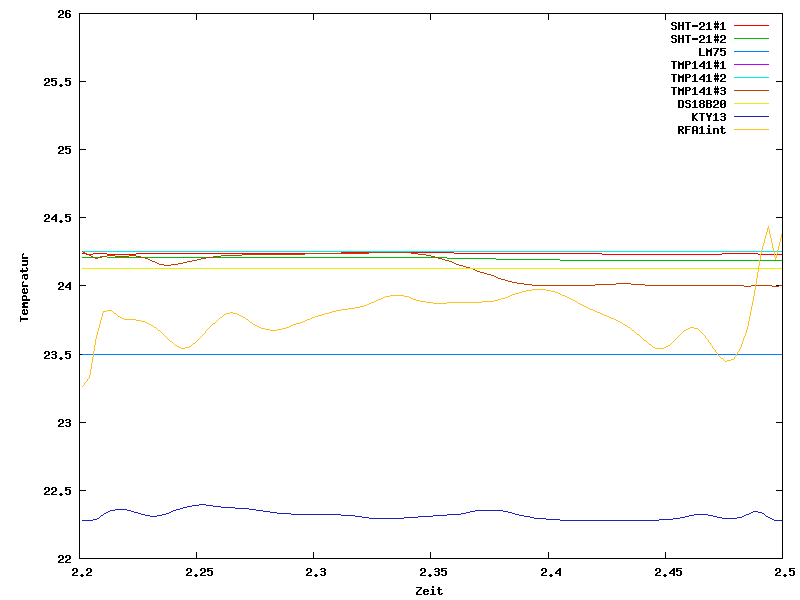
\includegraphics[width=\textwidth]{../smooth-stable.png}}%}
}

% ----------------------------------------

\frame{\frametitle{Messung im Klimaschrank}
\only<2>{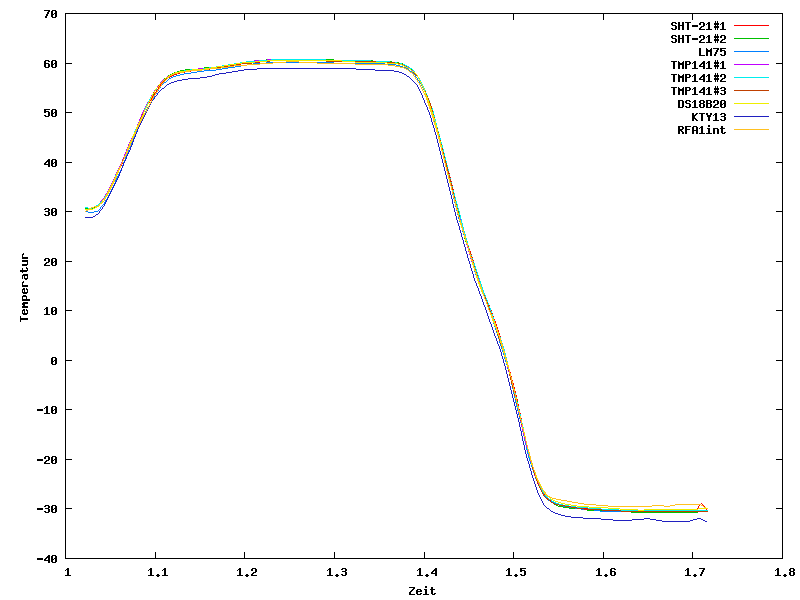
\includegraphics[width=\textwidth]{../schrank-komplett.png}}%}
\only<3>{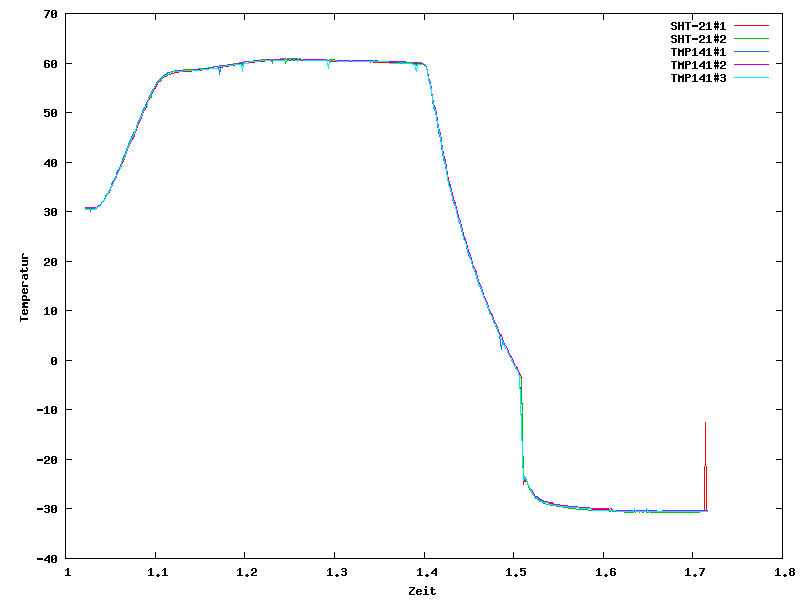
\includegraphics[width=\textwidth]{../schrank-sht-tmp.png}}%}
\only<4>{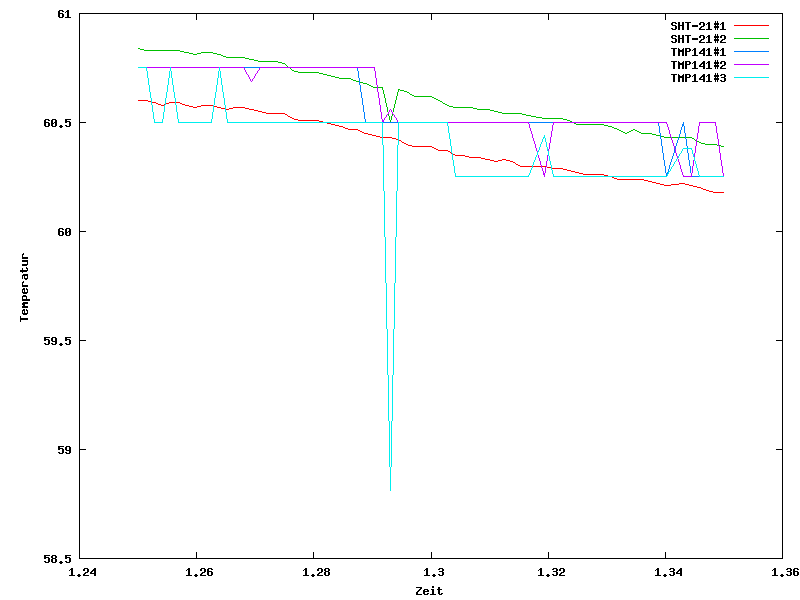
\includegraphics[width=\textwidth]{../schrank-sht-tmp-detail.png}}%}
}

% ----------------------------------------

\section{Schlussfolgerungen}
\frame{\frametitle{Schlussfolgerungen}
\Head{Temperaturmessung} \pause
\begin{itemize}
\item größte Abweichung: unkalibrierter KTY13-6, aber konstant -1,8 K \pause
\item LM75: -0,7 K, (ist mit ± 3K spezifiziert) \pause
\item alle anderen sehr eng gemeinsam gruppiert \pause
\item ATmega128RFA1: schlechte direkte Auflösung (1,13 K), aber gute
  Mittelwertbildung; Offset ca. -0,5 K, aber Gradient bei -30 °C \pause
\item SHT-21: Genauigkeit eines guten Laborthermometers, Nutzung als
  Referenz und für hohe Ansprüche \pause
\item TMP141 haben gutes Preis-/Leistungsverhältnis bei ansprechender
  Genauigkeit \pause
\end{itemize}

\Head{Feuchtigkeitsmessung} \pause
\begin{itemize}
\item kein Vergleich, nur SHT-21 selbst; gegenseitige Abweichung $< 1 \%$\,RH
\end{itemize}
}

% ----------------------------------------

% server slides

\section{Datenauswertung auf dem PC}
\frame{\frametitle{Datenauswertung auf dem PC I}
\begin{figure}
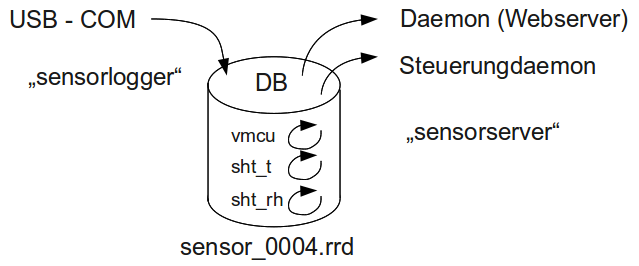
\includegraphics[width=0.6\textwidth]{../rrd_db.png}
\end{figure}

\begin{itemize}
  \item \Head{Speicherung in Round Robin Datenbank (rrdtool Projekt)}
 	\begin{itemize}
 	\item Aktuelle Messwerte am interessantesten
 	\item pro Sensor (\texttt{addr}) eine Datenbank (\texttt{.rrd}-File)
 	\item je Meßgröße (\texttt{vmcu}, \texttt{sht\_t}) eine oder mehrere Round Robin Archive möglich
 	\end{itemize}

  \item \Head{Sensorlogger}
	\begin{itemize}
	\item Gateway $\rightarrow$ USB  $\rightarrow$ Interface
	\item Python-Daemon zur Erfassung einlaufender Daten
	\item Lesen der Daten vom ser. Interface (\texttt{/dev/ttyUSB0}):
	\texttt{addr:4, acc: [27, 13, 80], sht\_rh: 26902, vmcu: 2744, sht\_t: 25800}
	\end{itemize}
\end{itemize}
}

% ----------------------------------------

\frame{\frametitle{Datenauswertung auf dem PC II}
\begin{figure}
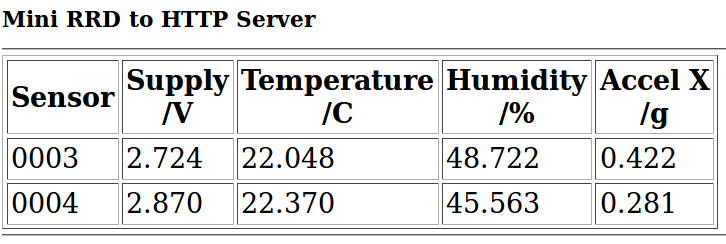
\includegraphics[width=0.8\textwidth]{../tableserver.png}
\end{figure}

\Head{Sensorserver}
\begin{itemize}
	\item Applikationen zur Auswertung (Visualisierung)
	\item Zugriff auf RRD-Datenbank-Daten
	\item Einfacher Mini-HTTP-Server in Python
	\item Erzeugen von Tabellen mit aktuellen Werten (\texttt{tableserver})
	\item Grafiken aus RRD-Datenbanken (Visualisierung) (\texttt{sensorserver})
\end{itemize}
}

% ----------------------------------------
\section{Datenlogger}
\begin{frame}[fragile]
\frametitle{Datenlogger (Prinzip) - \texttt{sensorlogger.py}}

\begin{verbatim}
import rrdtool
import serial
def rrd_create(tstamp, addr, **kwargs):
  # ... prep to create new .rrd file
  rrdtool.create(r.dbname, *args)

def rrd_update(tstamp, addr, **kwargs):
  # ... prep to update .rrd file with new data
  rrdtool.update(r.dbname, arg)
\end{verbatim}
\end{frame}

\begin{frame}[fragile]
\frametitle{Datenlogger (Prinzip) - \texttt{sensorlogger.py}}

\begin{verbatim}
sport = serial.Serial(SPORT, BAUD)
sport.open()
  while 1:
    try:
      x = sport.readline().strip()
      y = eval("dict(%s)" % x)  # well, it's a demo!
      y["tstamp"] = int(time.time())
      if not SENSORS.has_key(y["addr"]):
        rrd_create(**y)
      rrd_update(**y)
    except:
      print "ERROR:", sys.exc_info()
\end{verbatim}
\end{frame}

% ----------------------------------------

\section{Web-Server}
\begin{frame}[fragile]
\frametitle{Web-Server}
\begin{figure}
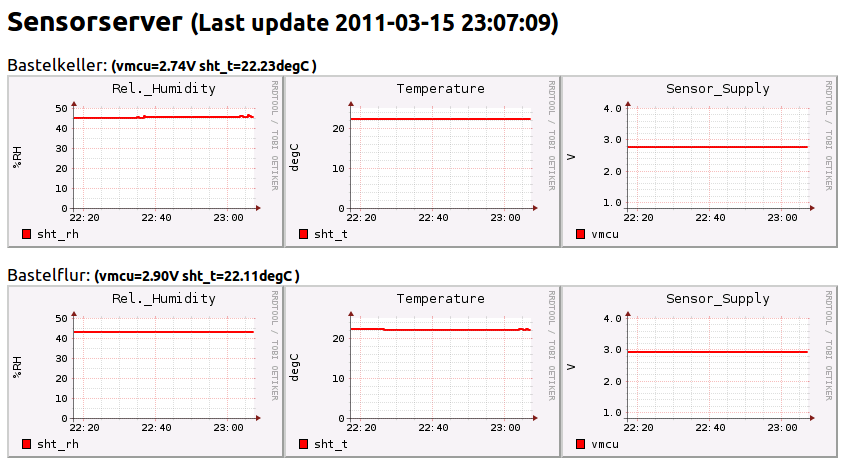
\includegraphics[width=0.9\textwidth]{../sensorserver_graph.png}
\end{figure}


\begin{verbatim}
  python sensorlogger.py -p /dev/ttyUSB0 -D
  python sensorserver.py -v
  python tableserver.py -v
\end{verbatim}

\end{frame}

% ----------------------------------------
\section{Ausblick}
\begin{frame}
\frametitle{Ausblick}

\begin{itemize}

\item Demo: Erfassung, Übertragung und Visualisierung der Sensordaten
\item Hinzufügen von Benachrichtigungsfunktionen (SMS, E-Mail)
\item Optimierung des Energieverbrauchs
	\begin{itemize}
	\item  Optimierung des Sensor-Datenprotokolls
	\item  Verlängerung der Knoten-Schlafzustände
	\end{itemize}

\item Steuerungsfunktionalität (Bidirektionaler Datenverkehr)
	\begin{itemize}
	\item  Sensorknoten empfangen Daten
	\item  Bidirektionaler Datenverkehr
	\end{itemize}

\item Einbindung in Heimautomatisierungssystem
	\begin{itemize}
	\item  Sensorknoten + Gateway (Modbus Protokoll?)
	\item  Framework zur Prozessvisualisierung, Steuerungsfunktionalität
	\end{itemize}
\end{itemize}
\end{frame}

% ----------------------------------------

\section{Danksagung}
\begin{frame}
\frametitle{Danksagung}

Wir möchten uns bei den folgenden Firmen und Personen
für die Unterstützung bei diesem Vortrag bedanken.

\vspace{0.3 cm}

\textbf{Herrn Daniel Thiele}
für die vielen Freizeitstunden bei Entwicklung und
Aufbau der RadioFaro-Module.

\vspace{0.3 cm}

\begin{figure}

\includegraphics[width=0.6\textwidth]{../sensirion_logo.jpg}
\end{figure}
für die großzügige Bemusterung mit digitalen Feuchtesensoren
vom Typ SHT21.
\texttt{http://www.sensirion.com}

\vspace{0.3 cm}

\begin{figure}

\includegraphics[width=0.6\textwidth]{../ibdt_logo.png}
\end{figure}
für die Bereitstellung der Muse231-Prototypen.
\texttt{http://www.ib-dt.de/}

\end{frame}

% ----------------------------------------
\begin{frame}
\frametitle{Referenzen}

\begin{itemize}
\item \texttt{http://uracoli.nongnu.org/clt2011/index.html}
	\begin{itemize}
	\item Quelltexte zur Demo (Knoten, Gateway, Daemons)
	\item Links zu weiteren Quellen
	\end{itemize}

\item \texttt{http://uracoli.nongnu.org}
	\begin{itemize}
	\item Projektwebseite
	\end{itemize}

\item {\small\texttt{http://lists.nongnu.org/mailman/listinfo/uracoli-devel}}%
	\begin{itemize}
	\item Entwickler Mailingliste
	\end{itemize}

\item \texttt{http://www.sax.de/~joerg/tiny230}
	\begin{itemize}
	\item Dokumentation Tiny230 Board
	\end{itemize}

\item \texttt{http://www.uracoli.de/radiofaro.html}
	\begin{itemize}
	\item Dokumentation RadioFaro Board
	\end{itemize}

\item \texttt{http://www.ib-dt.de}
	\begin{itemize}
	\item Entwicklerseite des Muse231 Prototyps
	\end{itemize}
\end{itemize}

\end{frame}

% TOC page (can be jumped to from PDF menu)

\begin{frame}
\tableofcontents
\end{frame}

\end{document}
